\documentclass{article} % Tipo de documento

\usepackage[utf8]{inputenc} % Permite el uso de caracteres del Español

\usepackage[T1]{fontenc}

\usepackage{graphicx}

% Carátula del Artículo  

\title{Reporte de Actividad 3}

\author{Brenda Leyva Amaya}

\date{14 de febrero, 2018}
 

\begin{document}

\maketitle % Crea el título


\section{Introducción}

	La presente actividad tiene como fin el llevar a la práctica diferentes maneras de realizar gráficos utilizando las nuevas herramientas que tenemos, Jupyter Notebook y las bibliotecas de manipulación de datos de Python. El tema con el cual se abordó la actividad es la medición de propiedades de la atmósfera con el apoyo de sondeos por globos meteorológicos. Para poder entonces contextualizar correctamente las actividades que se llevaron a cabo a continuación se incluye la información general principal del tema del cual se desprenden los datos estudiados y algunos resultados obtenidos. 

\section{Fundamentos.}

No será hasta finales de dicho siglo XIX y principios del XX, cuando surgen en todo el mundo las llamadas Estaciones Aerológicas, iniciándose y generalizándose las mediciones de los parámetros atmosféricos a diferentes alturas con ayuda de instrumentos que son elevados por medio de globos y cometas. Su fin era el estudio de las capas bajas y medias de la atmósfera para trazar a diversas alturas las cartas sinópticas, necesarias para predecir el tiempo en dichas zonas, a los ya por entonces pilotos de globos libres, dirigibles y de los primitivos aviones. Los sondeos se hacían, dependiendo del grado de estudio deseado, con ayuda de globos o cometas.
\vspace{0.5 cm}

Los tipos de globos utilizados para los sondeos podían ser:
\vspace{0.5 cm}

\textbf{Globos pilotos:} Es el método más simple de estudio aerológico y se usaba cuando se quería medir la velocidad y dirección del viento a diferentes alturas. Su nombre proviene de la costumbre de lanzar un globo pequeño a la atmósfera antes del lanzamiento de un globo tripulado para estimar la dirección del viento.
\vspace{0.5 cm}

\textbf{Globos sondas:} Globo libre no tripulado que transportaba un aparato (meteorógrafo) que registra continuamente las variaciones de la presión, temperatura y humedad relativa conforme se elevaba; observaciones desde tierra, permitían calcular la velocidad y dirección del viento a diferentes altitudes. Al llegar a una determinada altura la disminución de presión hacía explotar el globo y el meteorógrafo caía, teniendo que ser localizado con posterioridad para obtener los registros. Se empleaban para los sondeos dos globos unidos, de manera que al estallar uno de ellos, el otro sirviera, al permanecer hinchado, de paracaídas del meteorógrafo. Este método de sondeo ha perdurado hasta hoy en día, con los lógicos adelantos tecnológicos (radiosondas).
\vspace{0.5 cm}

\textbf{Globo-Cometa y Globos libres:} Estos globos eran empleados en los Servicios de Aerostación Militar con el propósito de realizar observaciones de los campos de batalla, en algunos de los vuelos de entrenamiento se llevaban meteorógrafos con el fin de realizar observaciones. Como alternativa o complemento a estas observaciones con globos se empleaban cometas.
\vspace{0.5 cm}

"Las ventajas que según Mr. Rotch tienen las cometas sobre los globos sondas para el estudio de las capas bajas y medias del aire son:
\vspace{0.5 cm}

1. Economía de gastos de instalación y experimentación.
\vspace{0.5 cm}

2. Seguridad en la altura a que se verifican las observaciones.
\vspace{0.5 cm}

3. Perfecta ventilación de los meteorógrafos empleados.
\vspace{0.5 cm}

El único inconveniente que tiene el sistema, es el de exigir el concurso del viento, lo cual hace preciso su complemento de globos cometas cautivos, para días de calma. El primer país en reconocer el potencial de las cometas en la investigación de la atmósfera fue Estados Unidos, en concreto en el Observatorio de Blue Hill (Massachusetts). A finales del siglo XIX, coincidiendo con la aparición de las cometas de tipo celular, su por entonces director A. Lawrence Rotch fija las bases y sistemática de la observación con ayuda de cometas. El 4 de agosto de 1894 consiguió elevar a 430 m un termógrafo, siguió a esta primera experiencia un continuo estudio para perfeccionar tanto los instrumentos registradores y los tipos de cometas, consiguiendo, en 1900, elevar un meteorógrafo a la considerable altura de 7000 m.
\vspace{0.5 cm}

Rápidamente el uso de las cometas en observaciones meteorológicas se extiende por otros países como Francia, en el Observatorio de Trappes, Alemania, el Observatorio Marítimo de Hamburgo y el Observatorio de Lindenberg y otros observatorios nacionales. El 1 de agosto de 1919, en el Observatorio de Lindenberg, se elevó un tren de ocho cometas meteorológicas tipo "Schirmkastendrachen". Después de 18 horas de elevación y 15 Km de cuerda de piano, como hilo, alcanzó los 9740 m. de altitud, récord que ha permanecido imbatible hasta ahora.
\vspace{0.5 cm}

Debido a que se necesitaba llegar a mayores alturas, al peligro de que se produjeran descargas eléctricas a través de los hilos, a la aparición de los primeros aviones y a la mejora de los Globos Sonda, las cometas entraran en desuso. Se dejaron de utilizar en la década de los treinta del siglo XX. Los globos que se utilizan actualmente son una versión modernizada de sus antecesores aquí mencionados, llevando a mediciones más finas y a mayores alturas que en el siglo pasado. 


\section{Análisis de datos.}

Al llevar a cabo esta actividad se obtuvieron una serie de datos que contenían ruido. Existían caracteres y lineas sin información que no permitía la correcta lectura e interpretación de los datos. Así dichos datos se debierón analizar e identificar aquellos elementos que entorpecían la lectura y estos a su vez fueron removidos del listado para poder proceder a realizar las actividades solicitadas.
\vspace{0.5 cm}

Adicionalmente algunos datos fueron identificados por el sistema como "integer" esto no nos permitía la correcta creación de los gráficos y se debió utilizar la función "astype" para llevar a cabo el cambio de integer a float y poder procesar la información.

\section{Resultados.}

A manera de resultados se agregan a continuación las diferentes gráficas que se crearon con los datos obtenidos, el lugar analizado fue Budapest y se tomarón el mes de Junio y de Diciembre para hacer comparativos correspondientes. 
\vspace{0.5 cm}

Comenzamos con la observación de la variación de la presión con respecto a la altura. 

 \begin{center}
 	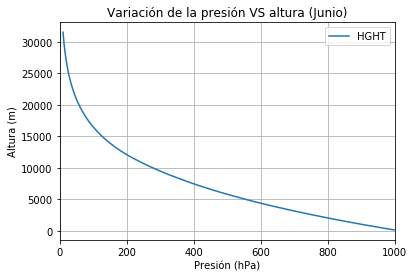
\includegraphics[width=8cm]{1.png}
 \end{center}


 \begin{center}
 	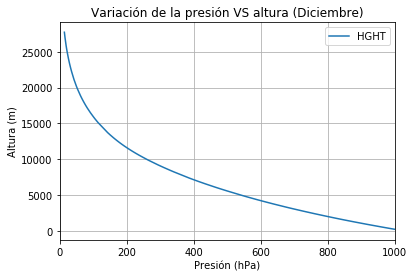
\includegraphics[width=8cm]{2.png}
 \end{center}

A continuación se generan las gráficas correspondientes que permitan analizar la variación de la temperatura con respecto a la altura. Aquí se observa que las variaciones de temperatura no se comportan de manera lineal, contrario a esto existen grandes inconsistencias y comportamiento inestable, ya que en diferentes alturas como vimos en la actividad anterior existen diferentes circunstancias que generan variaciones en la temperatura. 

 \begin{center}
 	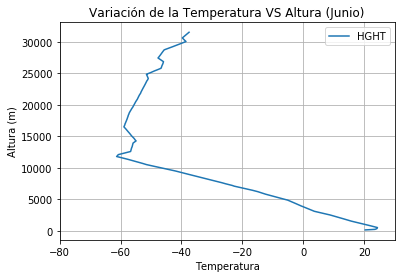
\includegraphics[width=9cm]{3.png}
 \end{center}


\begin{center}
 	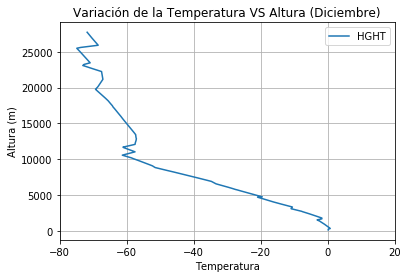
\includegraphics[width=9cm]{4.png}
 \end{center}

Con respecto a la temperatura y a la temperatura de rocío se observa que el comportamiento es muy similar, lo cual es esperado e intuitivo en cierta manera. 

\begin{center}
 	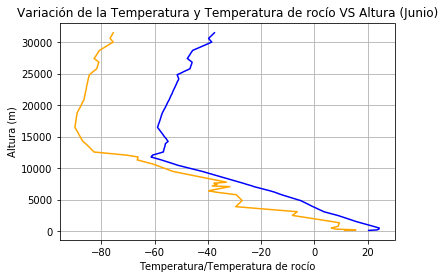
\includegraphics[width=9cm]{5.png}
 \end{center}


\begin{center}
 	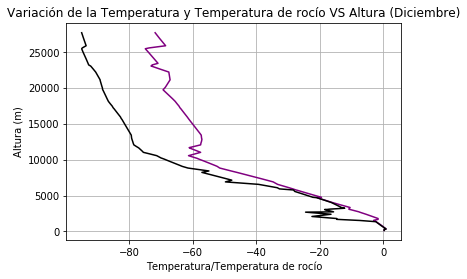
\includegraphics[width=9cm]{6.png}
 \end{center}

En el análisis de la rapidez de los vientos se puede observar una notoria diferencia en el comportamiento entre el mes de Junio y el de Diciembre, en Diciembre los vientos tienen menos variaciones extremas que en el mes de Junio, el cual presenta tanto aumentos como disminuciones extremos.

\begin{center}
 	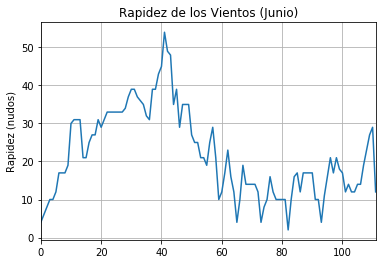
\includegraphics[width=8cm]{7.png}
 \end{center}
 
 
 \begin{center}
 	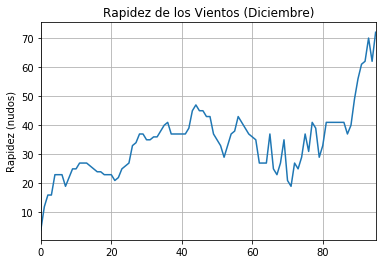
\includegraphics[width=8cm]{8.png}
 \end{center}
 
 La humedad relativa respecto a la altura tiene un comportamiento "extraño", hasta aproximadamente 12,000 metros de altura se observa que en verano existen una mayor cantidad de variaciones en el nivel de humedad mientras que en invierno tiene menos picos y alteraciones en su gráfica. A partir de esos aproxiamadamente 12,000 metros se observa un estancamiento de la humedad con tendencia a valores cercanos a cero. 
 
 \begin{center}
 	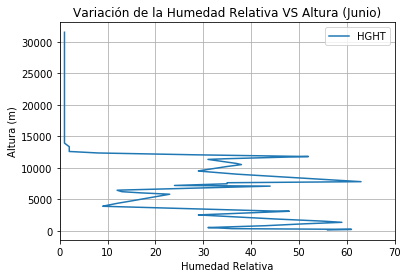
\includegraphics[width=8cm]{9.png}
 \end{center}
 
 
 \begin{center}
 	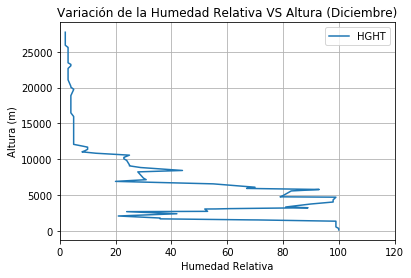
\includegraphics[width=8cm]{10.png}
 \end{center}


\section{Conclusión.}

A manera de conclusión es pertinente mencionar que la actividad se llevó a cabo con un grado de dificultad en cierto sentido bajo. Las metas de dicha sesión se fueron cumpliendo como era esperado y el producto final se espera puede cumplir con los requisitos que se tenían para el mismo.
\vspace{0.5 cm}

Es interesante poder gráficar diferentes datos de manera tan rápida y eficiente, esto ayuda de gran manera a su interpretación pues la parte visual ayuda a obtener conclusiones mucho más rápido que el simple análisis matemático de las direntes relaciones entre los datos obtenidos. 
\vspace{0.5 cm}

Será interesante ver los alcances que estas herramientas tienen con otro tipo de datos y contextos, y como se podrá ir aplicando a las diferentes necesidades que se presente a lo largo de nuestra preparación profesional.


\section*{Bibliografía.}

Suay Belenguer, J. M. (2003, December 06). Sondeos de la atmósfera con globos y cometas a principios del siglo XX. Retrieved February 13, 2018, from http://casanchi.com/fis/suaybelenguer01.htm 

\section*{Apéndice:}

\hspace{0.45 cm} ¿Cuál es tu opinión general de esta actividad?
\vspace{0.5 cm}

** Fué una actividad muy agradable y permitió obtener más práctica con la graficación y manipulación de datos.
\vspace{0.5 cm}

¿Qué fue lo que más te agradó? ¿Lo que menos te agradó?
\vspace{0.5 cm}

** Me agradó la información que consulté para establecer los fundamentos y además dentro del uso de Jupyter y Python que en esta ocasión el formato en el cual se leían los datos no era el óptimo y se tuvieron que aplicar nuevas herramientas como el cambiar un dato integer a un float. 
\vspace{0.5 cm}


¿Que consideras que aprendiste en esta actividad? 
\vspace{0.5 cm}

** Nuevas herramientas para graficación, modificación de tipo de datos y algunos conceptos nuevos en meteorología.
\vspace{0.5 cm}


¿Qué le faltó? ¿O le sobró?  
\vspace{0.5 cm}

** No logré identificar alguna deficiencia en la actividad.
\vspace{0.5 cm}


¿Que mejoras sugieres a la actividad?
\vspace{0.5 cm}

** No tengo una opinión al respecto, creo que la actividad fué buena y el tiempo con el que se contó para realizarla fue adecuado. 
\vspace{0.5 cm}


 
\end{document}